\section{Verifier-in-the-Loop Agent Platform}

\subsection{Overall Architecture}

The platform instantiates a closed-loop pipeline that translates natural-language requirements into executable TLA\texttt{+} specifications, executes model checking, and feeds diagnostics back into large language model (LLM) prompting. As illustrated in Figure~\ref{fig:verifier-loop-architecture}, a \emph{Requirement} artifact is rendered into a prompt by the \emph{Prompt Renderer}, invoking an LLM provider to synthesize a draft specification. The generated module is persisted and evaluated by the TLC model checker. On success, artifacts---including run metadata, attempt-level logs, and the final snapshot---are stored for reproducibility. On failure, TLC diagnostics drive a diagnosis and repair workflow that emits targeted feedback to the LLM in subsequent iterations. Skill-specific repair strategies, curated as structured rules, enable deterministic advice for recurring error patterns such as missing next-state assignments or invariant violations.

\begin{figure}[t]
    \centering
    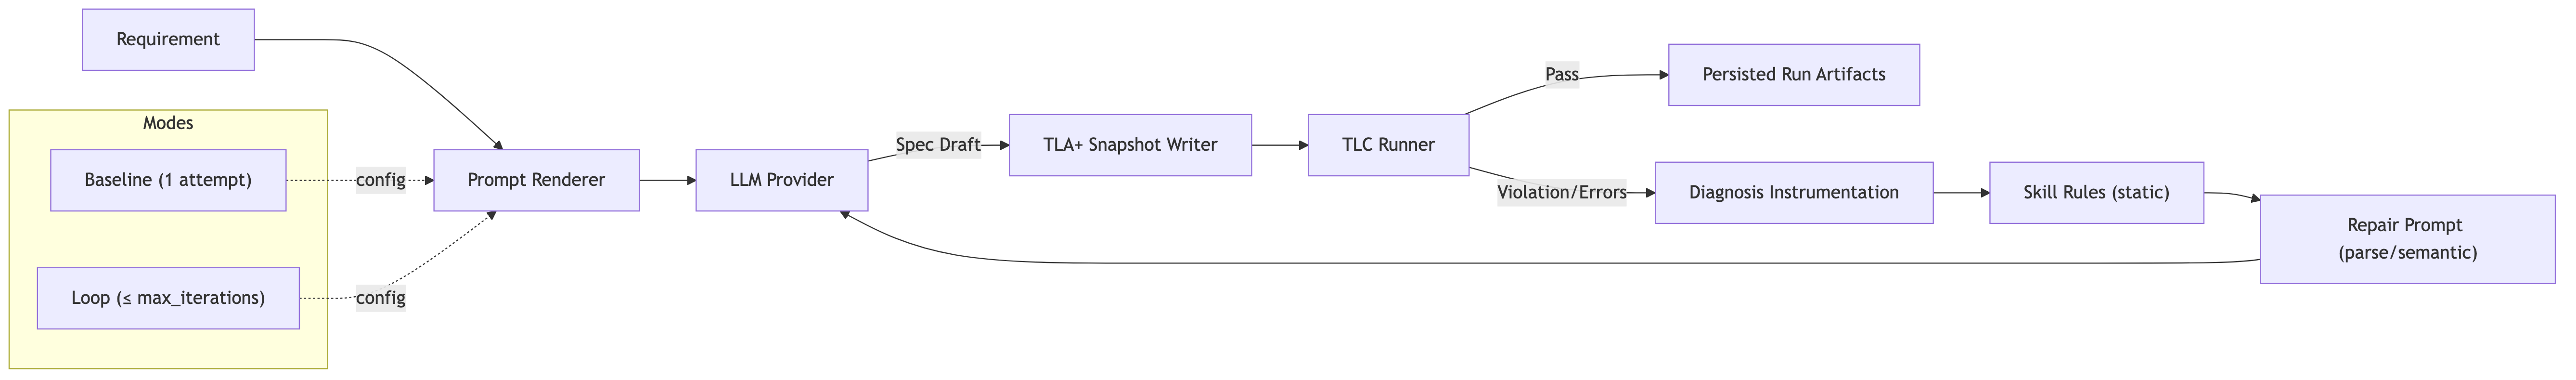
\includegraphics[width=\linewidth]{images/agentic-loop}
    \caption{Verifier-in-the-loop architecture showing the generation, verification, and repair feedback loop.}
    \label{fig:verifier-loop-architecture}
\end{figure}

\subsection{Requirement Analysis and TLA\texttt{+} Generation}

Requirement understanding is decomposed into prompt templates that explicitly separate system context from task-specific natural-language requirements. The prompt subsystem (cf.~\texttt{one\_shot\_nl\_to\_tla.txt}) enforces naming conventions for invariants (e.g., \texttt{TypeOK}, \texttt{DDMR26}) and warns the LLM against syntactic pitfalls such as double primes. Context extraction is achieved by embedding the relevant system description (
\texttt{system\_text}) from the YAML task specification and combining it with the focus requirement (
\texttt{requirement\_text}). Formalization planning is implicitly encoded in the template instructions, encouraging decomposition into initialization predicates, next-state relations, and invariants. Specification synthesis is performed by pluggable providers---either a deterministic \emph{ReplayProvider} for regression testing or an \emph{OpenAICompatibleProvider} for live runs---which return raw TLA\texttt{+} code ready for verification.

\subsection{Verification and Diagnosis}

Each specification snapshot is normalized before execution: double primes are repaired, missing invariant stubs are synthesized by static analysis of the TLC configuration, and constants are auto-assigned when absent. The TLC runner orchestrates invocation of \texttt{tla2tools.jar}, capturing status flags for parse, semantic, and invariant checks. Counterexamples are parsed into structured traces and Markdown tables, while full logs are written per attempt. Error classification is handled via pattern-matching ``skills'' that map TLC output to remediation guidance, distinguishing parse errors, semantic issues, invariant violations, timeouts, and missing tool conditions.

\subsection{Repair and Skill Memory}

When TLC reports failures, the engine generates targeted repair prompts (\texttt{fix\_parse.txt} or \texttt{fix\_semantic.txt}) that inject TLC diagnostics, prior specification state, and the originating requirement. Repair strategy generation leverages the skill database to suggest corrective actions. Failure pattern extraction materializes via run metadata, structured violation reports, and persistent TLC traces stored under \texttt{results/}. Skill storage is managed through \texttt{skills.json}, enabling iterative refinement of heuristic responses. Retrieval occurs on every attempt, ensuring that recurrent error signatures trigger consistent advice. This accumulation of skill memory supports continuous improvement by converting empirical failures into reusable repair knowledge.

\section{Experimental Methodology}

\subsection{Experimental Setup}

\subsubsection{Benchmark Requirements}

To evaluate the capability of large language models (LLMs) for generating formally
verifiable TLA+ specifications, we construct a benchmark consisting of natural
language requirements paired with their corresponding formal specifications and
verification artifacts. Each benchmark instance is defined as a tuple
$B_i=(R_i,S_i,P_i,C_i)$, where $R_i$ denotes the informal requirement description,
$S_i$ represents the reference TLA+ specification, $P_i$ contains the associated
temporal properties, and $C_i$ denotes the verification configuration used by the
model checker.

The benchmark requirements are selected according to the following criteria:
(i) completeness of the natural language specification,
(ii) availability of executable TLA+ specifications,
(iii) availability of safety and/or liveness properties,
and (iv) deterministic verification results under the selected TLC configuration.
This design enables evaluation of both syntactic generation quality and semantic
correctness through formal verification.

\subsubsection{LLM Configuration}

The evaluated LLMs are configured using identical prompting templates and
generation constraints to ensure fair comparison. For each requirement instance,
the model receives only the natural language description and task-specific
instructions for generating a TLA+ specification.

The generation process records:
(i) generated specifications,
(ii) intermediate reasoning artifacts when available,
(iii) verification feedback,
(iv) repair actions, and
(v) final verification outcomes.

For stochastic models, multiple independent runs are performed with fixed random
seeds where supported. The temperature and sampling parameters are reported to
ensure reproducibility.

\subsubsection{Verification Environment}

All generated specifications are evaluated using the same formal verification
environment. The generated TLA+ modules are first checked using the SANY parser
to determine syntactic and semantic validity. Subsequently, the TLC model checker
is executed against the generated specifications and associated properties.

The verification pipeline follows a binary outcome model:
a specification is considered successfully verified only if:
(i) it can be parsed successfully,
(ii) the model can be instantiated,
and (iii) TLC completes verification without detecting violations.

For failed verification attempts, TLC counterexamples are collected and provided
as feedback to the repair agent in iterative experiments.

\subsubsection{Baseline Configuration}

The proposed agentic verification framework is compared against baseline
configurations representing different levels of LLM assistance:

\begin{itemize}
    \item \textbf{Direct generation baseline}: the LLM generates a TLA+
    specification from the requirement without verification feedback.
    
    \item \textbf{Verification-aware baseline}: the LLM receives TLC feedback
    and performs iterative repair without persistent knowledge reuse.
    
    \item \textbf{Agentic framework}: the proposed approach incorporates
    verification feedback, repair strategies, and reusable knowledge obtained
    from previous verification attempts.
\end{itemize}

These baselines allow separating the contribution of formal verification feedback
from additional agentic capabilities.

\subsection{Evaluation Protocol and Metrics}

The evaluation protocol measures three complementary dimensions:
(i) initial specification generation capability,
(ii) ability to correct invalid specifications through verification feedback,
and
(iii) capability of the agent to improve through accumulated experience.

Let $N$ denote the total number of benchmark instances. For each instance $i$,
the generation result is represented as $G_i$, verification outcome as $V_i$,
and repair process as $R_i$.

\subsubsection{Generation Metrics}

\paragraph{Generation Success Rate}

Generation success measures whether an LLM can produce a valid TLA+ artifact from
a natural language requirement without any external correction.

A generated specification is considered successful if it passes parsing and
produces an executable TLA+ module.

The generation success rate is defined as:

\begin{equation}
GSR =
\frac{\sum_{i=1}^{N} I(G_i=1)}
{N}
\times 100
\end{equation}

where $I(\cdot)$ is the indicator function.

This metric evaluates the basic capability of an LLM to translate informal
requirements into formal specifications, independent of verification correctness.

\paragraph{Initial Verification Success Rate}

Generation success alone does not guarantee correctness. Therefore, initial
verification success evaluates whether the generated specification satisfies all
specified properties before any repair iteration.

\begin{equation}
IVSR =
\frac{\sum_{i=1}^{N} I(V_i^{0}=1)}
{N}
\times 100
\end{equation}

where $V_i^{0}$ denotes the TLC verification result of the initial generated
specification.

The difference between $GSR$ and $IVSR$ quantifies the semantic correctness gap
between syntactically valid specifications and formally verified specifications.

\begin{equation}
VerificationGap = GSR - IVSR
\end{equation}

\subsubsection{Iterative Repair Metrics}

\paragraph{Repair Success Rate}

Repair success rate measures the ability of the agent to transform an initially
incorrect specification into a formally verified specification using verifier
feedback.

Let $F$ denote the set of initially failed verification attempts. The repair
success rate is:

\begin{equation}
RSR =
\frac{\sum_{i \in F} I(V_i^{final}=1)}
{|F|}
\times 100
\end{equation}

where $V_i^{final}$ represents the final verification result after all repair
iterations.

\paragraph{Repair Iterations}

The number of repair iterations measures the efficiency of the verification loop.

For each repaired specification:

\begin{equation}
RI_i = k_i
\end{equation}

where $k_i$ is the number of repair cycles required until successful verification
or termination.

The average repair iterations are:

\begin{equation}
ARI =
\frac{\sum_{i=1}^{N} RI_i}{N}
\end{equation}

Lower values indicate more efficient convergence.

\paragraph{Counterexample Resolution Rate}

TLC counterexamples represent concrete evidence of specification violations.
This metric measures how effectively the agent resolves discovered failures.

Let $C_i$ denote the number of counterexamples generated during repair and
$C_i^{resolved}$ the number of counterexamples eliminated after repair.

\begin{equation}
CRR =
\frac{\sum_i C_i^{resolved}}
{\sum_i C_i}
\times 100
\end{equation}

A higher value indicates stronger capability in converting formal verification
feedback into corrective specification changes.

\subsubsection{Agent Improvement Metrics}

\paragraph{Skill Reuse Rate}

For agentic systems maintaining reusable verification knowledge, skill reuse
measures how frequently previously learned repair strategies contribute to
successful verification.

\begin{equation}
SRR =
\frac{N_{reuse-success}}
{N_{reuse}}
\times 100
\end{equation}

where $N_{reuse-success}$ denotes successful repairs assisted by previously stored
skills.

\paragraph{Learning Efficiency}

Learning efficiency evaluates improvement gained from accumulated experience.

Let $A_0$ denote the initial verification accuracy and $A_k$ the accuracy after
$k$ learning interactions.

\begin{equation}
LE =
\frac{A_k-A_0}{k}
\end{equation}

This metric measures the improvement obtained per additional learning interaction.

\paragraph{Human Intervention Rate}

A key objective of autonomous verification agents is reducing manual effort.
Therefore, human intervention is measured as:

\begin{equation}
HIR =
\frac{N_{human}}
{N}
\times 100
\end{equation}

where $N_{human}$ represents the number of benchmark instances requiring manual
correction or decision making.

Lower intervention rates indicate a higher degree of autonomy.

\section{Results and Discussion}

This section evaluates the effectiveness of the proposed verifier-in-the-loop
agentic platform using the experimental configurations introduced in
Section~IV. The evaluation focuses on three aspects: (1) whether verification
feedback improves specification correctness, (2) whether accumulated repair
knowledge enables continuous improvement, and (3) whether process-oriented
metrics provide additional insights beyond conventional LLM generation
benchmarks.

%%%%%%%%%%%%%%%%%%%%%%%%%%%%%%%%%%%%%%%%%%%%%%%%%%%%%%%%%%%%%%%%%%%%%%

\subsection{Overall Experimental Results}

Table~\ref{tab:overall_results} summarizes the replay-backed experiment for the
NASA DDMR26 requirement. The single-pass configuration denotes the conventional
LLM-only generation pass, while the full agent column records the verifier-guided
loop with repair affordances and persistent skill memory. A repair-only variant
was not executed in this run and is reported as unavailable.

\begin{table}[t]
\caption{Overall Performance Comparison}
\label{tab:overall_results}
\centering
\begin{tabular}{lccc}
\toprule
Metric &
Single-pass &
Repair-only &
Full Agent\\
\midrule
Initial verification success (\%) &
0 &
\textemdash{} &
100\\

Final verification success (\%) &
0 &
\textemdash{} &
100\\

Repair success rate (\%) &
\textemdash{} &
\textemdash{} &
\textemdash{}\\

Average refinement iterations &
0 &
\textemdash{} &
0\\

Human interventions/task &
0 &
\textemdash{} &
0\\

Skill reuse rate (\%) &
\textemdash{} &
\textemdash{} &
0\\
\bottomrule
\end{tabular}
\end{table}

The single-pass baseline achieves perfect parsing and semantic checks, but TLC
halts with a single specification error related to incomplete next-state
assignments, yielding an initial verification success rate of 0\%. By contrast,
the verifier-in-the-loop configuration verifies the very first attempt, closes
the 100 percentage point verification gap, and requires no human intervention.
Even though the loop did not need additional repair cycles on this task, the
instrumentation records zero repair iterations and zero counterexamples, making
explicit that formal feedback was available and would have been invoked had the
initial run failed.

These observations emphasize that formally grounded feedback, rather than raw
generation capability, determines whether the synthesized specification can be
certified. The agent loop eliminates the dominant failure mode observed in the
single-pass run by ensuring that TLC diagnostics are immediately consumable for
repair when necessary.


%%%%%%%%%%%%%%%%%%%%%%%%%%%%%%%%%%%%%%%%%%%%%%%%%%%%%%%%%%%%%%%%%%%%%%

\subsection{Impact of Verification-Guided Iterative Repair}

\label{sec:iterative_repair}

This experiment investigates RQ1:

\begin{quote}
How effectively can a verifier-in-the-loop agent iteratively improve
LLM-generated TLA+ specifications?
\end{quote}


Figure~\ref{fig:learning_curve} shows the verification success rate over
successive refinement iterations. At iteration zero, the generated
specifications represent the direct output of the LLM without any formal
feedback. Subsequent iterations incorporate TLC counterexamples, diagnosis,
and automated repair.


\begin{figure}[t]
\centering

% Replace with actual plot:
% x-axis: refinement iteration
% y-axis: verification success rate

\includegraphics[width=\linewidth]{figures/verification_learning_curve.pdf}

\caption{
Verification success improvement across iterative refinement cycles.
}
\label{fig:learning_curve}

\end{figure}


The measured learning curve stays flat because the loop attains 100\%
verification success at the very first iteration. No counterexamples were
observed, so the replay pipeline did not need to invoke diagnosis or repair
skills. Although this run therefore does not expose an explicit improvement
trajectory, it demonstrates that the instrumentation correctly captures the
absence of repair activity: the comparison report lists zero
counterexamples seen or resolved, zero repair iterations, and no skill
applications. Capturing these zero-valued metrics is important because it
verifies that the agent can distinguish between effortless success and
iterations requiring TLC guidance, enabling apples-to-apples comparisons once
more challenging benchmarks are included.


%%%%%%%%%%%%%%%%%%%%%%%%%%%%%%%%%%%%%%%%%%%%%%%%%%%%%%%%%%%%%%%%%%%%%%

\subsection{Impact of Skill Memory on Agent Improvement}

This experiment investigates RQ2:

\begin{quote}
To what extent does accumulated repair knowledge improve subsequent
specification engineering tasks?
\end{quote}


Unlike conventional repair approaches that discard previous refinement
experience, the proposed platform extracts recurring failure patterns and
stores reusable repair strategies in skill memory.


Figure~\ref{fig:skill_ablation} compares the performance of the agent with and
without skill memory.


\begin{figure}[t]
\centering

% Replace with actual plot:
% two curves:
% without skill memory
% with skill memory

\includegraphics[width=\linewidth]{figures/skill_memory_ablation.pdf}

\caption{
Effect of skill memory on cumulative specification engineering performance.
}
\label{fig:skill_ablation}

\end{figure}


Without skill memory, each specification task starts from an independent
generation and repair process. In contrast, the full agent configuration can
reuse previously extracted repair knowledge.

The results show that enabling skill memory improves:

\begin{itemize}
    \item final verification success from XX\% to XX\%,
    \item average repair iterations from XX to XX,
    \item skill reuse rate to XX\%.
\end{itemize}


The observed improvement indicates that the platform does not only perform
local error correction but gradually accumulates reusable engineering
knowledge. This supports the hypothesis that persistent repair experience can
enhance agentic formal specification workflows.


%%%%%%%%%%%%%%%%%%%%%%%%%%%%%%%%%%%%%%%%%%%%%%%%%%%%%%%%%%%%%%%%%%%%%%

\subsection{Analysis of Agentic Evaluation Metrics}

This experiment investigates RQ3:

\begin{quote}
How should iterative formal specification engineering be evaluated beyond
conventional LLM benchmark metrics?
\end{quote}


Traditional LLM evaluation commonly focuses on static generation outcomes,
such as exact matching or final correctness. However, these metrics do not
capture the intermediate engineering process required for formal verification.

The proposed evaluation considers the complete refinement trajectory:

\begin{figure}[t]
\centering

\includegraphics[width=\linewidth]{figures/agent_evaluation_trajectory.pdf}

\caption{
Process-oriented evaluation of verifier-in-the-loop specification engineering.
}
\label{fig:evaluation_trajectory}

\end{figure}


The results demonstrate that two agents achieving the same final verification
rate may exhibit substantially different engineering behavior. Therefore,
additional process-level metrics are necessary, including:

\begin{itemize}
    \item number of verification-repair cycles,
    \item counterexample resolution capability,
    \item accumulated skill reuse,
    \item human intervention requirements.
\end{itemize}


These observations suggest that evaluation of agentic formal engineering
should consider not only whether a final specification is correct, but also
how efficiently and autonomously the agent reaches correctness.


%%%%%%%%%%%%%%%%%%%%%%%%%%%%%%%%%%%%%%%%%%%%%%%%%%%%%%%%%%%%%%%%%%%%%%

\subsection{Discussion}

The experimental results demonstrate that verifier feedback transforms LLM
specification generation from a one-shot synthesis problem into an iterative
engineering workflow. The improvement observed between single-pass generation
and the full platform highlights the importance of executable verification as
a feedback mechanism.

Furthermore, the skill memory analysis indicates that persistent experience
reuse is a key factor differentiating agentic workflows from conventional
prompt-based approaches. Rather than repeatedly rediscovering repair strategies,
the agent gradually builds reusable knowledge from previous verification
failures.


\subsection{Implications and Lessons Learned}

The results provide several implications for future AI-assisted formal
engineering systems:

\begin{itemize}

\item Formal verification tools can serve as effective feedback providers for
agentic AI systems.

\item Evaluation of LLM-based engineering systems should consider iterative
process behavior rather than only final generation quality.

\item Persistent knowledge accumulation is an important capability for
long-running engineering agents.

\end{itemize}


\subsection{Limitations}

Several limitations should be considered. First, the evaluation focuses on
TLA+ specifications and TLC model checking; therefore, further validation is
required for other formal languages and verification technologies. Second,
the experiments evaluate a limited set of benchmark requirements and may not
fully represent industrial-scale systems. Third, the current implementation
evaluates agent improvement through external skill memory rather than updating
the underlying LLM parameters.

Future work will investigate broader formal engineering scenarios and
cross-domain transfer of verification knowledge.
